% !TeX program = pdflatex
% Beamer slides derived from Chapter 5 (LQR Design via Quadratic Programming)
% Figures are referenced with the same relative paths as the lecture notes.

\documentclass[aspectratio=169,11pt]{beamer}

\usetheme{Madrid}
\usecolortheme{default}
\setbeamertemplate{navigation symbols}{}
\setbeamertemplate{caption}[numbered]

\usepackage{amsmath, amssymb, mathtools, bm}
\usepackage{graphicx}
\usepackage{grffile} % robust filenames (e.g., with spaces)
\usepackage{booktabs}
\usepackage{tikz}
\usetikzlibrary{patterns,shadings,arrows.meta,positioning}
\usepackage{listings}
\usepackage{microtype}

% Keep figure addresses compatible with the notes (slides assumed to live next to them).
\graphicspath{{./}{./Figures/}}
\DeclareGraphicsExtensions{.pdf,.png,.jpg,.jpeg}

% ---------- Convenience macros ----------
\newcommand{\R}{\mathbb{R}}
\newcommand{\T}{\top}
\newcommand{\norm}[1]{\left\lVert #1 \right\rVert}
\newcommand{\argmin}{\operatorname*{arg\,min}}
\newcommand{\blkdiag}{\operatorname{blkdiag}}
\newcommand{\vect}{\operatorname{vec}}

% Safe includegraphics: compiles even if figure files are not present in this environment.
\newcommand{\includegraphicssafe}[2][]{%
  \IfFileExists{#2}{\includegraphics[#1]{#2}}{%
    \IfFileExists{#2.pdf}{\includegraphics[#1]{#2.pdf}}{%
      \IfFileExists{#2.png}{\includegraphics[#1]{#2.png}}{%
        \fbox{\parbox[c][0.26\textheight][c]{0.92\linewidth}{\centering\small Figure file not found at\\\texttt{#2}\\(Place the slides next to the notes so the \texttt{Figures/} folder is available.)}}%
      }%
    }%
  }%
}

% Styling blocks for long-form explanations.
\setbeamercolor{block title}{fg=white,bg=black!70}
\setbeamercolor{block body}{bg=black!4,fg=black}
\setbeamercolor{block title alerted}{fg=white,bg=red!70!black}
\setbeamercolor{block body alerted}{bg=red!4,fg=black}
\setbeamercolor{block title example}{fg=white,bg=blue!70!black}
\setbeamercolor{block body example}{bg=blue!4,fg=black}

\title[LQR via QP]{LQR Design via Quadratic Programming\\\small (Chapter 5 in the MPC lecture notes)}
\author{\tiny { İbrahim Küçükdemiral}}
\date{\small March 2026}

\begin{document}

% ==============================================================
\begin{frame}
  \titlepage
\end{frame}


\begin{frame}{Where this chapter fits in the MPC story}
\begin{block}{Big picture}
Model Predictive Control (MPC) is, at its core, a repeated solution of a finite-horizon optimisation problem. LQR is the cleanest ``training ground'' for this idea because it is the same type of optimisation problem, but without inequality constraints.
\end{block}

\begin{block}{Why we do LQR \emph{via} Quadratic Programming here}
The classical textbook route introduces LQR through Riccati equations and dynamic programming. That route is efficient and elegant, but it can hide the optimisation structure that MPC solvers must handle.
In this chapter we instead assemble the whole trajectory problem into one quadratic programme (QP). This ``batch'' view makes the move to constrained MPC almost automatic: constraints simply become additional inequalities.
\end{block}
\end{frame}

\begin{frame}{Learning outcomes for a 3-hour lecture}
\begin{block}{By the end, you should be able to}
\begin{enumerate}
  \item Explain LQR as a finite-horizon optimisation problem, clearly identifying decision variables, cost terms, and equality constraints.
  \item Construct the sparse (simultaneous) QP formulation by stacking states and inputs, and interpret the structure of the Hessian and constraint matrices.
  \item Derive the KKT system and explain how solving it by back-substitution produces the Riccati recursion and a state-feedback law.
  \item Describe why the finite-horizon gains converge for time-invariant systems and derive the Discrete Algebraic Riccati Equation (DARE).
  \item Extend LQR from regulation to non-zero setpoint tracking and interpret the resulting affine control law as ``feedforward + feedback''.
\end{enumerate}
\end{block}
\end{frame}

\begin{frame}{Roadmap for today (3 hours)}
\begin{block}{Three lecture blocks (with short breaks)}
\begin{enumerate}
  \item \textbf{Finite-horizon LQR as an optimisation problem} (motivation, formulation, convexity).
  \item \textbf{Batch QP \& KKT} (stacking variables, sparse matrices, KKT system, Riccati recursion).
  \item \textbf{Beyond the finite horizon} (infinite-horizon LQR via DARE, stability intuition, setpoint tracking, MagLev case study).
\end{enumerate}
\end{block}

\begin{alertblock}{Reading tip}
If any derivation feels fast, pause and check each algebraic move. In optimal control, tiny sign mistakes produce big conceptual errors.
\end{alertblock}
\end{frame}

% ==============================================================
\section{Finite-horizon LQR as an optimisation problem}

\begin{frame}{System model and notation}
\begin{block}{Discrete-time linear dynamics}
We consider a (possibly time-varying) discrete-time linear system
\[
  x_{k+1} = A_k x_k + B_k u_k, \qquad k = 0,1,\dots,N-1,
\]
where the state is $x_k \in \R^n$ and the input is $u_k \in \R^m$. The horizon length is $N$, meaning we plan $N$ future steps and predict states up to $x_N$.
\end{block}

\begin{block}{What is known at optimisation time}
At each solve, the initial state $x_0$ is treated as known (measured or estimated). In an MPC setting, $x_0$ would be the current state estimate at the present sampling instant.
\end{block}
\end{frame}

\begin{frame}{What does ``optimal'' mean in LQR?}
\begin{block}{A quadratic cost that encodes trade-offs}
LQR chooses inputs by minimising a cost that penalises (i) being far from the desired operating point and (ii) using excessive control effort.
The standard finite-horizon quadratic cost is
\[
J = \frac{1}{2}x_N^\top Q_N x_N + \sum_{k=0}^{N-1}\left(\frac{1}{2}x_k^\top Q_k x_k + \frac{1}{2}u_k^\top R_k u_k\right).
\]
The matrices $Q_k$ and $Q_N$ shape how strongly we punish different state components, while $R_k$ shapes how expensive it is to use the actuator.
\end{block}

\begin{alertblock}{Interpretation that matters for MPC}
This is already the same structure used in most ``tracking MPC'' controllers. The only missing ingredient is inequality constraints such as $u_{\min}\le u_k\le u_{\max}$.
\end{alertblock}
\end{frame}

\begin{frame}{The optimisation problem (finite horizon)}
\begin{block}{Decision variables and constraints}
The optimisation chooses a whole future \emph{sequence} of inputs $\{u_0,\dots,u_{N-1}\}$ and the corresponding predicted states $\{x_1,\dots,x_N\}$. The problem is
\[
\begin{aligned}
\min_{x_{1:N},\,u_{0:N-1}}\quad & \frac{1}{2}x_N^\top Q_N x_N + \sum_{k=0}^{N-1}\left(\frac{1}{2}x_k^\top Q_k x_k + \frac{1}{2}u_k^\top R_k u_k\right)\\
\text{s.t.}\quad & x_0\;\text{given (measured)}\\
& x_{k+1} = A_k x_k + B_k u_k,\qquad k=0,\dots,N-1.
\end{aligned}
\]
\end{block}

\begin{block}{A key idea}
Although the dynamics are ``time-evolution equations'', in the optimisation they are just \emph{linear equality constraints} connecting variables.
\end{block}
\end{frame}

\begin{frame}{Convexity: why the weights matter}
\begin{block}{Why we impose $Q\succeq 0$ and $R\succ 0$}
For LQR to be well-posed and numerically stable, we usually require
\[
Q_k\succeq 0,\quad Q_N\succeq 0,\quad R_k\succ 0.
\]
Intuitively, $Q\succeq 0$ means ``the state penalty never rewards large states'', while $R\succ 0$ means ``using the actuator always costs something''. The strictness of $R\succ 0$ is important: it prevents the optimiser from choosing multiple equally good input sequences (or trying to use unbounded input energy to reduce state penalties).
\end{block}

\begin{alertblock}{Connection to a solver}
These conditions also guarantee the cost function is convex in the decision variables, so any local minimum is the global minimum. For a QP solver, this is the difference between a reliable, fast solve and an unstable numerical problem.
\end{alertblock}
\end{frame}

\begin{frame}{Why reformulate LQR as a quadratic programme?}
\begin{block}{Two equivalent viewpoints}
There are two mathematically equivalent ways to solve finite-horizon LQR:
\begin{enumerate}
  \item A \textbf{recursive} approach (Riccati recursion / dynamic programming), which exploits structure and is very efficient when there are no inequality constraints.
  \item A \textbf{batch (QP)} approach, which converts the entire trajectory problem into a single optimisation problem in standard form.
\end{enumerate}
\end{block}

\begin{block}{Why MPC cares about the batch view}
The moment we add inequality constraints, the elegant recursion breaks. MPC therefore uses the QP form as the standard computational representation, because constraints can be added and handled systematically.
\end{block}
\end{frame}

% ==============================================================
\section{Batch (sparse) QP formulation and KKT conditions}

\begin{frame}{From dynamic optimisation to static QP: the main trick}
\begin{block}{Stack everything into one vector}
The ``batch'' idea is simple: instead of thinking in time, we collect (stack) all future decision variables into one large vector and write both the cost and the dynamics using block matrices.
Once we do that, LQR becomes a standard quadratic programme of the form
\[
\min_{\zeta}\;\frac{1}{2}\zeta^\top H\zeta\quad\text{subject to}\quad \mathcal{C}\zeta=d.
\]
\end{block}

\begin{alertblock}{Why the word ``sparse'' keeps appearing}
If we stack variables in a clever order, the matrices $H$ and $\mathcal{C}$ have many zeros and a banded structure. Modern solvers exploit this sparsity to solve problems quickly even when $N$ is large.
\end{alertblock}
\end{frame}

\begin{frame}{The decision vector $\zeta$ (simultaneous / sparse form)}
\begin{block}{Interleaving inputs and states}
We keep $x_0$ outside the decision vector because it is a known constant at solve time. A useful ordering is
\[
\zeta = \begin{bmatrix} u_0^\top & x_1^\top & u_1^\top & x_2^\top & \cdots & u_{N-1}^\top & x_N^\top \end{bmatrix}^\top.
\]
This interleaving keeps constraints local: each dynamic constraint only touches a small neighbourhood of variables $(u_k, x_{k+1})$ and sometimes $x_k$.
\end{block}

\begin{block}{What this means in plain language}
The optimiser is now choosing the entire future input sequence \emph{and} the entire future state sequence simultaneously, while the equality constraints enforce that those choices are physically consistent.
\end{block}
\end{frame}

\begin{frame}{The Hessian matrix $H$: encoding the cost}
\begin{block}{Block-diagonal structure}
The cost is a sum of quadratic terms in each $u_k$ and each $x_k$. Because the variables are stacked, the Hessian becomes block diagonal:
\[
H = \blkdiag(R_0,\,Q_1,\,R_1,\,\dots,\,R_{N-1},\,Q_N).
\]
This is ``sparse'' because there are no cross-terms between different time instants in the standard LQR cost.
\end{block}

\begin{alertblock}{A subtle but important detail}
The term $\tfrac12 x_0^\top Q_0 x_0$ is constant because $x_0$ is known, so it does not affect the minimiser and we typically omit it from the batch cost.
\end{alertblock}
\end{frame}

\begin{frame}{The equality constraint matrix $\mathcal{C}$: encoding dynamics}
\begin{block}{Rewrite each dynamic step as a linear equation}
Starting from $x_{k+1}=A_k x_k + B_k u_k$, move all decision variables to the left:
\[
-A_k x_k - B_k u_k + x_{k+1} = 0.
\]
For $k=0$, the state $x_0$ is known, so we move it to the right:
\[
-B_0 u_0 + x_1 = A_0 x_0.
\]
Stacking these $N$ equations produces a big but structured linear system $\mathcal{C}\zeta=d$.
\end{block}
\end{frame}

\begin{frame}{The ``staircase'' structure (why it is solver-friendly)}
\begin{block}{Typical block form}
For clarity, in the time-varying case the stacked constraint matrix has the form
\[
\mathcal{C}=
\begin{bmatrix}
 B_0 & -I & 0 & 0 & \cdots & 0\\
 0 & A_1 & B_1 & -I & \cdots & 0\\
 \vdots & \vdots & \ddots & \ddots & \ddots & \vdots\\
 0 & 0 & \cdots & A_{N-1} & B_{N-1} & -I
\end{bmatrix},\qquad
d=\begin{bmatrix}-A_0x_0\\0\\\vdots\\0\end{bmatrix}.
\]
Every row block links only a few neighbouring variables, which is why the matrix looks like a staircase.
\end{block}

\begin{alertblock}{Computational takeaway}
Even though $\mathcal{C}$ can be very large, it is mostly zeros. Sparse linear algebra routines take advantage of this, which is why MPC can run in real time.
\end{alertblock}
\end{frame}

\begin{frame}{A concrete miniature example (build intuition)}
\begin{exampleblock}{Suppose $N=3$ and the system is LTI}
The decision vector is
\[
\zeta=\begin{bmatrix}u_0^\top&x_1^\top&u_1^\top&x_2^\top&u_2^\top&x_3^\top\end{bmatrix}^\top.
\]
The dynamics give three constraints:
\[
\begin{aligned}
-Bu_0 + x_1 &= Ax_0,\\
-Ax_1 - Bu_1 + x_2 &= 0,\\
-Ax_2 - Bu_2 + x_3 &= 0.
\end{aligned}
\]
\end{exampleblock}

\begin{block}{What to notice}
The second and third constraints link three ``neighbour'' variables $(x_k,u_k,x_{k+1})$. This locality is exactly what we exploit in both sparse QP solvers and in Riccati recursion.
\end{block}
\end{frame}

\begin{frame}{Standard QP form: what a solver expects}
\begin{block}{Equality-constrained QP (our current setting)}
An optimisation solver typically expects
\[
\min_{\zeta}\;\frac{1}{2}\zeta^\top H\zeta + f^\top\zeta
\quad\text{s.t.}\quad \mathcal{C}\zeta = d.
\]
For the simplest LQR regulation problem, $f=0$ because the cost has no linear terms.
\end{block}

\begin{alertblock}{Preview of MPC}
In constrained MPC, we add inequalities
\[
\mathcal{G}\zeta \le h,
\]
which represent actuator saturation, safety limits, rate limits, and many other physical realities.
This is why spending time on the batch QP view is not optional for MPC.
\end{alertblock}
\end{frame}

\begin{frame}{Optimality conditions via the Lagrangian}
\begin{block}{From constrained optimisation to equations}
To solve
\(\min \tfrac12\zeta^\top H\zeta\) subject to \(\mathcal{C}\zeta=d\),
we introduce Lagrange multipliers $\lambda$ and form the Lagrangian
\[
\mathcal{L}(\zeta,\lambda) = \frac12\zeta^\top H\zeta + \lambda^\top(\mathcal{C}\zeta-d).
\]
The multipliers enforce the dynamics, and they will later reveal a deep connection to ``costates'' in optimal control.
\end{block}
\end{frame}

\begin{frame}{KKT conditions in this equality-only case}
\begin{block}{Two conditions = one linear system}
Setting derivatives to zero gives:
\[
\nabla_{\zeta}\mathcal{L} = H\zeta + \mathcal{C}^\top\lambda = 0\quad\text{(stationarity)},
\]
\[
\nabla_{\lambda}\mathcal{L} = \mathcal{C}\zeta - d = 0\quad\text{(primal feasibility)}.
\]
Combining them yields the \textbf{KKT system}
\[
\begin{bmatrix}
H & \mathcal{C}^\top\\
\mathcal{C} & 0
\end{bmatrix}
\begin{bmatrix}
\zeta\\\lambda
\end{bmatrix}
=
\begin{bmatrix}
0\\d
\end{bmatrix}.
\]
\end{block}

\begin{alertblock}{Interpretation}
The KKT system is not ``mysterious''. It is simply the set of linear equations that make the gradient of the constrained problem vanish.
In MPC software, solving KKT-like systems (or closely related systems) is the main computational work.
\end{alertblock}
\end{frame}

\begin{frame}{Multipliers as ``shadow prices'' (intuition)}
\begin{block}{Why $\lambda$ matters beyond maths}
Each equality constraint represents a physical requirement: ``the predicted states must follow the model''. The multipliers $\lambda$ quantify how much the optimal cost would change if we perturbed those constraints.

In optimal control language, these multipliers behave like \emph{costates}: they propagate information backward in time about how future penalties influence the present.
\end{block}

\begin{exampleblock}{A concrete mental model}
If $\lambda_{k+1}$ is large in some direction, it means the optimiser is ``very sensitive'' to errors in the corresponding component of $x_{k+1}$. That sensitivity is what drives the feedback law to correct the state.
\end{exampleblock}
\end{frame}

\begin{frame}{Explicit KKT structure for a short horizon}
\begin{block}{Why the matrix stays sparse}
When the system is LTI and we use constant weights $(A,B,Q,R)$, the KKT matrix has a banded, repeating pattern.
The notes expand this structure for $N=4$ and show how blocks like $B^\top$ and $A^\top$ appear in $\mathcal{C}^\top$ while $-I$ appears because of the $x_{k+1}$ term.
\end{block}

\begin{alertblock}{Key message}
Even though the KKT matrix can be very large, it is not a random dense matrix. Its structure mirrors the time structure of the system.
That is exactly why specialised solvers (and Riccati recursion) can solve it efficiently.
\end{alertblock}
\end{frame}

% ==============================================================
\section{From KKT to Riccati recursion}

\begin{frame}{Two ways to solve the same linear system}
\begin{block}{Option A: Let a linear solver do it}
You can solve the KKT system directly with sparse linear algebra. This is essentially what many MPC QP solvers do internally, although they use extra tricks for inequalities.
\end{block}

\begin{block}{Option B: Solve it analytically by exploiting time structure}
If we exploit the staircase/banded structure, we can eliminate variables step-by-step. Doing this elimination carefully produces a backward recursion in the matrix $P_k$ and the gain $K_k$.
That recursion is the Riccati recursion.
\end{block}
\end{frame}

\begin{frame}{Start at the end of the horizon (terminal condition)}
\begin{block}{The last state equation}
When you take the derivative of the Lagrangian with respect to the terminal state $x_N$, you obtain a relation between the last multiplier and the terminal penalty.
For the standard quadratic terminal cost, it becomes
\[
\lambda_N = Q_N x_N.
\]
This is the ``boundary condition'' that starts the backward recursion.
\end{block}

\begin{alertblock}{Why the recursion runs backward}
Future penalties (at times close to $N$) influence what we do today. Mathematically, that influence travels backward through the multipliers and the matrix $P_k$.
\end{alertblock}
\end{frame}

\begin{frame}{Optimising the last input (a template step)}
\begin{block}{The stationarity condition for $u_{N-1}$}
The derivative with respect to $u_{N-1}$ has the form
\[
R\,u_{N-1} + B^\top\lambda_N = 0.
\]
Substituting $\lambda_N = P_N x_N$ and then using the dynamics $x_N = Ax_{N-1}+Bu_{N-1}$ produces
\[
(R + B^\top P_N B)u_{N-1} = -B^\top P_N A\,x_{N-1}.
\]
So the optimal last input is a linear feedback of the last state:
\[
u_{N-1} = -K_{N-1}x_{N-1},\qquad K_{N-1}=(R+B^\top P_N B)^{-1}B^\top P_N A.
\]
\end{block}
\end{frame}

\begin{frame}{Update the multiplier one step earlier (costate recursion)}
\begin{block}{Stationarity condition for $x_{N-1}$}
The derivative with respect to $x_{N-1}$ gives
\[
Qx_{N-1} - \lambda_{N-1} + A^\top \lambda_N = 0,
\qquad\Rightarrow\qquad
\lambda_{N-1} = Qx_{N-1} + A^\top\lambda_N.
\]
Substitute $\lambda_N=P_N x_N$ and then substitute $x_N=(A-BK_{N-1})x_{N-1}$.
You obtain
\[
\lambda_{N-1} = \bigl(Q + A^\top P_N(A-BK_{N-1})\bigr)x_{N-1}.
\]
This motivates defining $\lambda_{k}=P_k x_k$ and yields the recursion for $P_k$.
\end{block}

\begin{alertblock}{Core pattern}
\(\lambda_{k}=P_kx_k\) is not a guess; it is the structure that drops out of the optimality equations for quadratic costs and linear dynamics.
\end{alertblock}
\end{frame}

\begin{frame}{The Riccati recursion (finite horizon, LTI case)}
\begin{block}{Backward pass: compute $P_k$ and $K_k$}
For LTI systems with constant $A,B,Q,R$ and horizon $N$:
\begin{align*}
P_N &= Q_N,\\
K_k &= (R + B^\top P_{k+1}B)^{-1}B^\top P_{k+1}A,\\
P_k &= Q + A^\top P_{k+1}(A - BK_k),\qquad k=N-1,\dots,0.
\end{align*}
\end{block}

\begin{block}{Forward pass: apply the gains}
Once $K_k$ is known, the optimal policy is
\[
u_k = -K_k x_k,
\]
and we simulate the dynamics forward from $x_0$ to produce the optimal trajectory.
\end{block}
\end{frame}

\begin{frame}{Why the recursion is computationally attractive}
\begin{block}{What the recursion avoids}
The batch KKT system grows with horizon length $N$. Solving it by generic matrix factorisation would cost roughly like a large sparse linear solve.
The Riccati recursion avoids solving one giant system by instead solving a sequence of smaller problems of size $n\times n$ and $m\times m$.
\end{block}

\begin{exampleblock}{A practical way to say it}
Rather than inverting a huge matrix, we do:
\begin{itemize}
  \item A backward sweep that updates $P_k$ and $K_k$.
  \item A forward sweep that applies $u_k=-K_kx_k$.
\end{itemize}
Each sweep scales linearly with horizon length and exploits the problem structure.
\end{exampleblock}
\end{frame}

\begin{frame}{Equivalence: QP solution vs. Riccati solution}
\begin{block}{Same optimisation problem, different computational routes}
The batch QP and the Riccati recursion are not two different controllers. They are two different ways of solving the \emph{same} finite-horizon optimisation problem.
If you solved the QP and extracted the optimal sequence $(u_0,\dots,u_{N-1})$, then simulated forward, you would obtain exactly the same trajectory as using the Riccati gains.
\end{block}

\begin{alertblock}{Why we keep both viewpoints}
Riccati is the cleanest way to understand why LQR yields linear feedback.
QP is the cleanest way to understand how MPC solvers operate, especially when constraints enter.
\end{alertblock}
\end{frame}

\begin{frame}{Worked example: double integrator (setup)}
\begin{exampleblock}{A simple but important benchmark}
The discrete-time double integrator (position and velocity) is a standard testbed for optimal control.
With sampling time $h$, a common discretisation is
\[
A=\begin{bmatrix}1 & h\\ 0 & 1\end{bmatrix},\qquad
B=\begin{bmatrix}\tfrac12 h^2\\ h\end{bmatrix}.
\]
We typically choose $Q=I$ to penalise both position and velocity, and a scalar $R>0$ to penalise input energy.
\end{exampleblock}

\begin{block}{Why this example matters}
Even though the model is simple, it contains the key engineering feature of many systems: the input affects acceleration, so position cannot change instantly. The optimal policy therefore naturally balances speed of correction against control effort.
\end{block}
\end{frame}

\begin{frame}{Worked example: finite-horizon behaviour (figure)}
\begin{block}{What you should read from the plot}
In the finite-horizon solution, the controller ``plans'' to bring both states to the origin by the end of the horizon. Early on, it may apply a stronger input to reduce position error and then later applies smaller inputs to settle smoothly.
\end{block}

\begin{figure}
  \centering
  \includegraphicssafe[width=0.95\linewidth]{Figures/Finite\_LQR.pdf}
  \caption{Finite-horizon LQR for the double integrator (figure address preserved from the notes).}
\end{figure}
\end{frame}

\begin{frame}[fragile]{Implementation sketch: backward pass / forward pass}
\begin{block}{The algorithmic structure you should remember}
Almost every practical LQR implementation follows the same two-phase pattern:
\begin{enumerate}
  \item \textbf{Backward pass:} initialise $P_N=Q_N$, then iterate $k=N-1\to 0$ computing $K_k$ and $P_k$.
  \item \textbf{Forward pass:} simulate from $x_0$ using $u_k=-K_kx_k$.
\end{enumerate}
\end{block}

\begin{exampleblock}{A short MATLAB-like pseudo-code}
\begin{lstlisting}[language=Matlab,basicstyle=\ttfamily\small]
P{N+1} = QN;
for k = N:-1:1
  K{k} = (R + B'*P{k+1}*B) \ (B'*P{k+1}*A);
  P{k} = Q + A'*P{k+1}*(A - B*K{k});
end

x = x0;
for k = 1:N
  u = -K{k}*x;
  x = A*x + B*u;
end
\end{lstlisting}
\end{exampleblock}
\end{frame}

\begin{frame}{Checkpoint: questions you should be able to answer now}
\begin{block}{Conceptual checks}
\begin{enumerate}
  \item If we increase $R$ while keeping $Q$ fixed, why does the control signal become ``more conservative''?
  \item Why is $R\succ 0$ (strict) more important than $Q\succeq 0$ (non-strict) for uniqueness?
  \item In the batch QP, what role does the vector $d$ play, and why does it contain $x_0$?
\end{enumerate}
\end{block}

\begin{alertblock}{Short answers (for self-study)}
Increasing $R$ makes input energy expensive, so the optimiser tolerates larger state deviations. Strict positivity of $R$ avoids flat directions in input space. The vector $d$ injects the known initial condition into the stacked dynamics constraints.
\end{alertblock}
\end{frame}

% ==============================================================
\section{Infinite-horizon LQR and the DARE}

\begin{frame}{Why the infinite horizon is the default in practice}
\begin{block}{Regulation tasks do not ``end''}
Many engineering control tasks are not ``reach the origin at time $T$'' problems. They are ``keep the system near a desired operating point forever'' problems.
In such problems, we conceptually take $N\to\infty$.
\end{block}

\begin{block}{A surprising but useful fact}
For time-invariant $(A,B,Q,R)$, the finite-horizon Riccati recursion typically converges quickly: far from the terminal time, $P_k$ and $K_k$ become approximately constant.
This is the motivation for the infinite-horizon solution.
\end{block}
\end{frame}

\begin{frame}{Empirical convergence of $P_k$ (figure)}
\begin{block}{How to interpret the convergence plot}
As we run the backward recursion from $k=N$ to $k=0$, the entries of $P_k$ often approach steady values after only a modest number of steps.
The influence of the chosen terminal cost $Q_N$ fades as we move away from the end of the horizon.
\end{block}

\begin{figure}
  \centering
  \includegraphicssafe[width=0.48\linewidth]{Figures/Riccati Convergence}
  \caption{Convergence of the Riccati recursion (figure address preserved from the notes).}
\end{figure}
\end{frame}

\begin{frame}{From recursion to fixed point: the DARE idea}
\begin{block}{If it converges, it should satisfy a steady-state equation}
If $P_k$ converges as the horizon grows, then in the infinite-horizon limit we expect
\[
P_k = P_{k+1} = P
\]
for a constant matrix $P$.
Substituting this fixed-point assumption into the Riccati recursion converts the backward recursion into an algebraic equation.
\end{block}

\begin{alertblock}{Why this matters}
Instead of storing a time-varying sequence $\{K_k\}$, we can compute a single gain $K$ that is optimal for the infinite-horizon problem and is cheap to implement on embedded hardware.
\end{alertblock}
\end{frame}

\begin{frame}{The Discrete Algebraic Riccati Equation (DARE)}
\begin{block}{Derivation (compressed but explicit)}
Start with
\[
K = (R + B^\top P B)^{-1}B^\top P A.
\]
Insert this gain into
\[
P = Q + A^\top P (A - BK).
\]
After substitution and simplification, the infinite-horizon matrix $P$ satisfies
\[
P = Q + A^\top P A - A^\top P B (R + B^\top P B)^{-1}B^\top P A.
\]
This nonlinear matrix equation is the \textbf{Discrete Algebraic Riccati Equation}.
\end{block}

\begin{alertblock}{What ``nonlinear'' means here}
The unknown $P$ appears both linearly and inside the inverse term $(R+B^\top P B)^{-1}$. That is why we rely on specialised numerical algorithms to solve the DARE.
\end{alertblock}
\end{frame}

\begin{frame}{The infinite-horizon LQR controller}
\begin{block}{Once $P$ is known, everything becomes simple}
Solve the DARE for $P\succeq 0$ and compute
\[
K = (R + B^\top P B)^{-1}B^\top P A.
\]
Then the optimal infinite-horizon control law is
\[
u_k = -Kx_k.
\]
This is a static state-feedback controller: it does not explicitly depend on time, and it does not need to store a horizon of gains.
\end{block}

\begin{block}{Closed-loop dynamics}
With $u_k=-Kx_k$, the closed-loop system is
\[
x_{k+1} = (A-BK)x_k \;\triangleq\; A_{\mathrm{cl}}x_k.
\]
\end{block}
\end{frame}

\begin{frame}{Why LQR gives a stability guarantee}
\begin{block}{The key theorem (stated, not proven)}
Under standard assumptions (stabilisability of $(A,B)$ and detectability of $(Q^{1/2},A)$), the DARE has a unique stabilising solution $P\succeq 0$, and the resulting gain $K$ makes the closed-loop matrix $A_{\mathrm{cl}}=A-BK$ stable.
\end{block}

\begin{block}{What ``stable'' means in discrete time}
Discrete-time stability means all eigenvalues of $A_{\mathrm{cl}}$ lie strictly inside the unit circle:
\[
\rho(A_{\mathrm{cl}}) < 1.
\]
In other words, repeated multiplication by $A_{\mathrm{cl}}$ shrinks the state over time.
\end{block}

\begin{alertblock}{Engineering interpretation}
The cost function acts like a Lyapunov function. The Riccati solution constructs a function $V(x)=x^\top P x$ that decreases under the optimal feedback.
\end{alertblock}
\end{frame}

\begin{frame}{Computing $K$ in practice (MATLAB / toolbox view)}
\begin{block}{You rarely solve the DARE by hand}
In MATLAB, the standard call is
\[
[P, L, K] = \texttt{dare}(A,B,Q,R),
\]
which returns the DARE solution $P$, the closed-loop eigenvalues $L$, and the gain $K$.
\end{block}

\begin{block}{What to check after calling \texttt{dare}}
You should verify that the eigenvalues in $L$ have magnitudes less than one. If they do not, the likely causes are that the system is not stabilisable, the weights are ill-conditioned, or the discrete-time model is incorrect.
\end{block}
\end{frame}

\begin{frame}{Infinite-horizon example: double integrator (figure)}
\begin{block}{What changes compared to finite-horizon}
In the infinite-horizon case, a constant gain $K$ is used at every time step. The response is typically similar to the beginning of a long-horizon finite-horizon solution, because that is where the Riccati recursion has already converged.
\end{block}

\begin{figure}
  \centering
  \includegraphicssafe[width=0.95\linewidth]{Figures/InFinite\_LQR.pdf}
  \caption{Infinite-horizon LQR for the double integrator (figure address preserved from the notes).}
\end{figure}
\end{frame}

% ==============================================================
\section{LQR for non-zero setpoint tracking}

\begin{frame}{Regulation vs. tracking: what changes?}
\begin{block}{Regulation is ``drive to zero''}
So far, the objective has been to drive $x_k\to 0$. This is appropriate when the origin represents the desired operating point (after shifting coordinates appropriately).
\end{block}

\begin{block}{Tracking is ``drive to a non-zero equilibrium''}
In many applications, the desired operating point is non-zero, so we specify a target pair $(x_g,u_g)$ such that the system can stay there forever.
That pair must satisfy the equilibrium condition
\[
x_g = A x_g + B u_g.
\]
\end{block}
\end{frame}

\begin{frame}{Why the equilibrium input $u_g$ is essential}
\begin{exampleblock}{Intuition: hovering drone}
If a drone hovers at a fixed height, its vertical velocity is zero at equilibrium, but the thrust input is not zero.
The non-zero input is exactly what cancels gravity.
\end{exampleblock}

\begin{block}{General lesson}
When the physics includes constant disturbances or forces (gravity, steady loads, friction offsets, biases), the equilibrium input typically is not zero.
If we ignore this and only use feedback around the origin, the controller will ``fight'' the constant effect and we often get steady-state error.
\end{block}
\end{frame}

\begin{frame}{Deviation (error) variables: the standard trick}
\begin{block}{Shift the coordinates so the target becomes the origin}
Define deviation variables
\[
\tilde{x}_k \triangleq x_k - x_g,\qquad \tilde{u}_k \triangleq u_k - u_g.
\]
The goal ``$x_k \to x_g$'' becomes ``$\tilde{x}_k\to 0$''.
\end{block}

\begin{block}{Derive the deviation dynamics}
Subtract the equilibrium equation from the dynamics:
\[
\tilde{x}_{k+1} = x_{k+1}-x_g = (Ax_k+Bu_k) - (Ax_g+Bu_g) = A\tilde{x}_k + B\tilde{u}_k.
\]
So the deviation system has the \emph{same} $A$ and $B$ matrices.
\end{block}
\end{frame}

\begin{frame}{The affine control law (feedforward + feedback)}
\begin{block}{Design LQR on the deviation system}
For the deviation variables, the standard LQR law is
\[
\tilde{u}_k = -K\tilde{x}_k.
\]
Substitute $\tilde{u}_k=u_k-u_g$ and $\tilde{x}_k=x_k-x_g$:
\[
u_k - u_g = -K(x_k-x_g)
\quad\Rightarrow\quad
u_k = u_g - K(x_k-x_g).
\]
\end{block}

\begin{alertblock}{Interpretation you should remember}
The control action has a baseline term $u_g$ that maintains the operating point, and a correction term $-K(x_k-x_g)$ that reacts to deviations.
This ``affine'' structure is exactly what appears again in offset-free MPC formulations.
\end{alertblock}
\end{frame}

\begin{frame}{How to compute $(x_g,u_g)$ from an output reference}
\begin{block}{When the reference is given as an output target}
Often we want $y_{\mathrm{ref}}$ rather than $x_g$. With output equation $y=Cx$, the steady-state target must satisfy
\[
x_g = Ax_g + Bu_g,\qquad y_{\mathrm{ref}} = Cx_g.
\]
These can be solved together as a linear system:
\[
\begin{bmatrix} I-A & -B\\ C & 0\end{bmatrix}
\begin{bmatrix} x_g\\ u_g\end{bmatrix}
=
\begin{bmatrix} 0\\ y_{\mathrm{ref}}\end{bmatrix}.
\]
\end{block}

\begin{alertblock}{Feasibility requirement}
The matrix must be invertible. A common sufficient condition is that the number of inputs equals the number of tracked outputs and the steady-state equations are well-conditioned.
In constrained settings, the same idea becomes the ``target calculator'' problem in MPC.
\end{alertblock}
\end{frame}

\begin{frame}{Case study preview: why MagLev is a good example}
\begin{block}{Magnetic levitation is non-linear and open-loop unstable}
The MagLev plant has strongly nonlinear physics (magnetic force varies as $(i/y)^2$) and behaves like an inverted pendulum: without feedback it diverges from equilibrium.
This makes it an excellent example for showing two important ideas:
\begin{enumerate}
  \item Why a non-zero equilibrium input is essential.
  \item Why designing LQR on a linearisation can still work well on the nonlinear plant near the operating point.
\end{enumerate}
\end{block}
\end{frame}

\begin{frame}{MagLev model (nonlinear dynamics)}
\begin{block}{Nonlinear state-space model}
Let $x_1=y$ be the gap and $x_2=\dot{y}$ be the vertical velocity. With a simplified magnetic force model $F_{\mathrm{mag}} = C\,(u/y)^2$, the dynamics can be written as
\[
\dot{x}_1 = x_2,\qquad
\dot{x}_2 = g - \frac{C}{m}\left(\frac{u}{x_1}\right)^2.
\]
At equilibrium, acceleration is zero, so magnetic force balances weight.
\end{block}

\begin{alertblock}{What makes this hard}
The input appears as $u^2$ divided by $x_1^2$. This nonlinearity means there is no globally linear controller that is ``perfect'', and we must rely on local design and feedback robustness.
\end{alertblock}
\end{frame}

\begin{frame}{MagLev equilibrium and linearisation (conceptual steps)}
\begin{block}{Step 1: equilibrium input}
Choose a nominal operating gap $y_{\mathrm{eq}}$. At equilibrium, $\dot{x}_2=0$ so
\[
C\left(\frac{u_{\mathrm{eq}}}{y_{\mathrm{eq}}}\right)^2 = mg
\quad\Rightarrow\quad
u_{\mathrm{eq}} = y_{\mathrm{eq}}\sqrt{\frac{mg}{C}}.
\]
\end{block}

\begin{block}{Step 2: linearise about the equilibrium}
Compute Jacobians to obtain a continuous-time linear model $\dot{x}=A_c x + B_c u$ around the operating point. The notes show that one entry of $A_c$ is positive, which indicates open-loop instability and motivates feedback design.
\end{block}
\end{frame}

\begin{frame}{MagLev schematic (from the notes)}
\begin{figure}
\centering
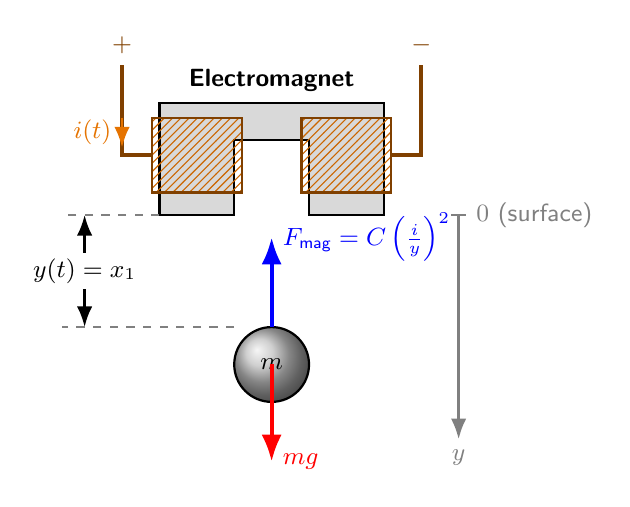
\begin{tikzpicture}[>=Latex, thick, scale=0.95, font=\small\sffamily]

  % Electromagnet
  \fill[fill=gray!30, draw=black] (-1.5, 0) -- (1.5, 0) -- (1.5, -1.5) -- (0.5, -1.5) -- (0.5, -0.5) -- (-0.5, -0.5) -- (-0.5, -1.5) -- (-1.5, -1.5) -- cycle;

  % Coils
  \fill[pattern=north east lines, pattern color=orange!80!black, draw=orange!50!black] (-1.6, -1.2) rectangle (-0.4, -0.2);
  \fill[pattern=north east lines, pattern color=orange!80!black, draw=orange!50!black] (0.4, -1.2) rectangle (1.6, -0.2);

  % Wires
  \draw[orange!50!black, line width=1.5pt] (-1.6, -0.7) -- (-2, -0.7) -- (-2, 0.5) node[above] {$+$};
  \draw[orange!50!black, line width=1.5pt] (1.6, -0.7) -- (2, -0.7) -- (2, 0.5) node[above] {$-$};
  \draw[->, orange!90!black, line width=1pt] (-2, -0.2) -- (-2, -0.6) node[midway, left] {$i(t)$};
  \node at (0, 0.3) {\textbf{Electromagnet}};

  % Ball
  \shade[ball color=gray!50] (0, -3.5) circle (0.5cm);
  \draw (0, -3.5) circle (0.5cm);
  \node at (0, -3.5) {$m$};

  % Forces
  \draw[->, red, line width=1.5pt] (0, -3.5) -- (0, -4.8) node[right] {$mg$};
  \draw[->, blue, line width=1.5pt] (0, -3.0) -- (0, -1.8) node[right] {$F_{\text{mag}} = C\left(\frac{i}{y}\right)^2$};

  % Reference lines
  \draw[dashed, gray] (-1.5, -1.5) -- (-2.8, -1.5);
  \draw[dashed, gray] (-0.5, -3.0) -- (-2.8, -3.0);

  % Gap
  \draw[<->, black, line width=1pt] (-2.5, -1.5) -- (-2.5, -3.0) node[midway, fill=white, inner sep=2pt] {$y(t)=x_1$};

  % Axis
  \draw[->, gray, line width=1pt] (2.5, -1.5) -- (2.5, -4.5) node[below] {$y$};
  \draw[gray, thick] (2.4, -1.5) -- (2.6, -1.5) node[right] {$0$ (surface)};
\end{tikzpicture}
\caption{Schematic of the magnetic levitation system (redrawn from the chapter).}
\end{figure}
\end{frame}

\begin{frame}{MagLev tracking result (figure)}
\begin{block}{What to look for}
The top plot shows the gap moving from the initial equilibrium (10 mm) to the new target (12 mm) with a smooth response and no overshoot.
The bottom plot shows the control current settling to a \emph{non-zero} steady value, which is exactly the feedforward equilibrium current required to balance gravity at the new gap.
\end{block}

\begin{figure}
  \centering
  \includegraphicssafe[width=0.78\linewidth]{Figures/Maglev.pdf}
  \caption{MagLev setpoint tracking (figure address preserved from the notes).}
\end{figure}
\end{frame}

\begin{frame}{What this case study teaches (and what MPC adds)}
\begin{block}{Lessons}
\begin{enumerate}
  \item \textbf{Equilibrium matters:} without the feedforward term $u_g$, even a good feedback gain will generally produce steady-state error when constant forces or biases are present.
  \item \textbf{Local models can work:} an LQR designed on a linearisation can stabilise and track well on a nonlinear plant, provided we operate near the linearisation point and sample fast enough.
  \item \textbf{Why MPC is next:} MagLev actuators have current limits, and the gap has safety limits. LQR does not enforce these explicitly. MPC will incorporate them as inequalities.
\end{enumerate}
\end{block}

\begin{alertblock}{Bridge to the next chapter}
If you can express your problem as ``quadratic cost + linear dynamics + (in)equalities'', you are already in MPC territory.
\end{alertblock}
\end{frame}

% ==============================================================
\section{Summary and self-study prompts}

\begin{frame}{Chapter summary (what to remember)}
\begin{block}{The essential chain of ideas}
\begin{enumerate}
  \item Finite-horizon LQR is an optimisation problem: quadratic cost, linear dynamics constraints, known initial state.
  \item By stacking variables, LQR becomes a sparse equality-constrained QP, which is the computational template for MPC.
  \item The KKT conditions produce a structured linear system; solving it by back-substitution yields the Riccati recursion.
  \item In time-invariant settings, the Riccati recursion converges, leading to a fixed point: the DARE and a constant optimal gain.
  \item For non-zero setpoints, shift to deviation variables to obtain an affine control law with feedforward and feedback.
\end{enumerate}
\end{block}
\end{frame}

\begin{frame}{Self-study exercises (with guidance)}
\begin{block}{Exercise 1: weight tuning}
Pick a simple 2-state system (e.g., the double integrator) and simulate LQR responses for three choices of $(Q,R)$:
one that prioritises speed, one that prioritises small inputs, and one that prioritises damping.
Write one paragraph explaining how the plots reflect the cost terms.
\end{block}

\begin{block}{Exercise 2: build the batch matrices}
For $N=2$ and LTI $(A,B)$, write out $\zeta$, $H$, and $\mathcal{C}$ explicitly by hand.
Then check that $\mathcal{C}\zeta=d$ indeed enforces $x_1=Ax_0+Bu_0$ and $x_2=Ax_1+Bu_1$.
\end{block}
\end{frame}

\begin{frame}{Preview: what changes when we go from LQR to MPC?}
\begin{block}{Only one new ingredient: inequalities}
MPC uses the same prediction model and the same kind of quadratic objective, but it adds constraints such as
\[
u_{\min}\le u_k\le u_{\max},\qquad x_{\min}\le x_k\le x_{\max}.
\]
These constraints turn the problem into a constrained QP that must be solved repeatedly in receding horizon fashion.
\end{block}

\begin{alertblock}{Key message}
If you understand today's batch formulation and KKT logic, you already understand the mathematical engine of linear MPC.
\end{alertblock}
\end{frame}

\begin{frame}
\centering
\Huge Questions?
\end{frame}

\end{document}
